\begin{figure}[h!]
    \centering
    \caption{Minimum wage levels in the US by jurisdiction, 2010--2019}
    \label{fig:mw_policies}

    \begin{subfigure}{.7\textwidth}
        \caption{State policies}
        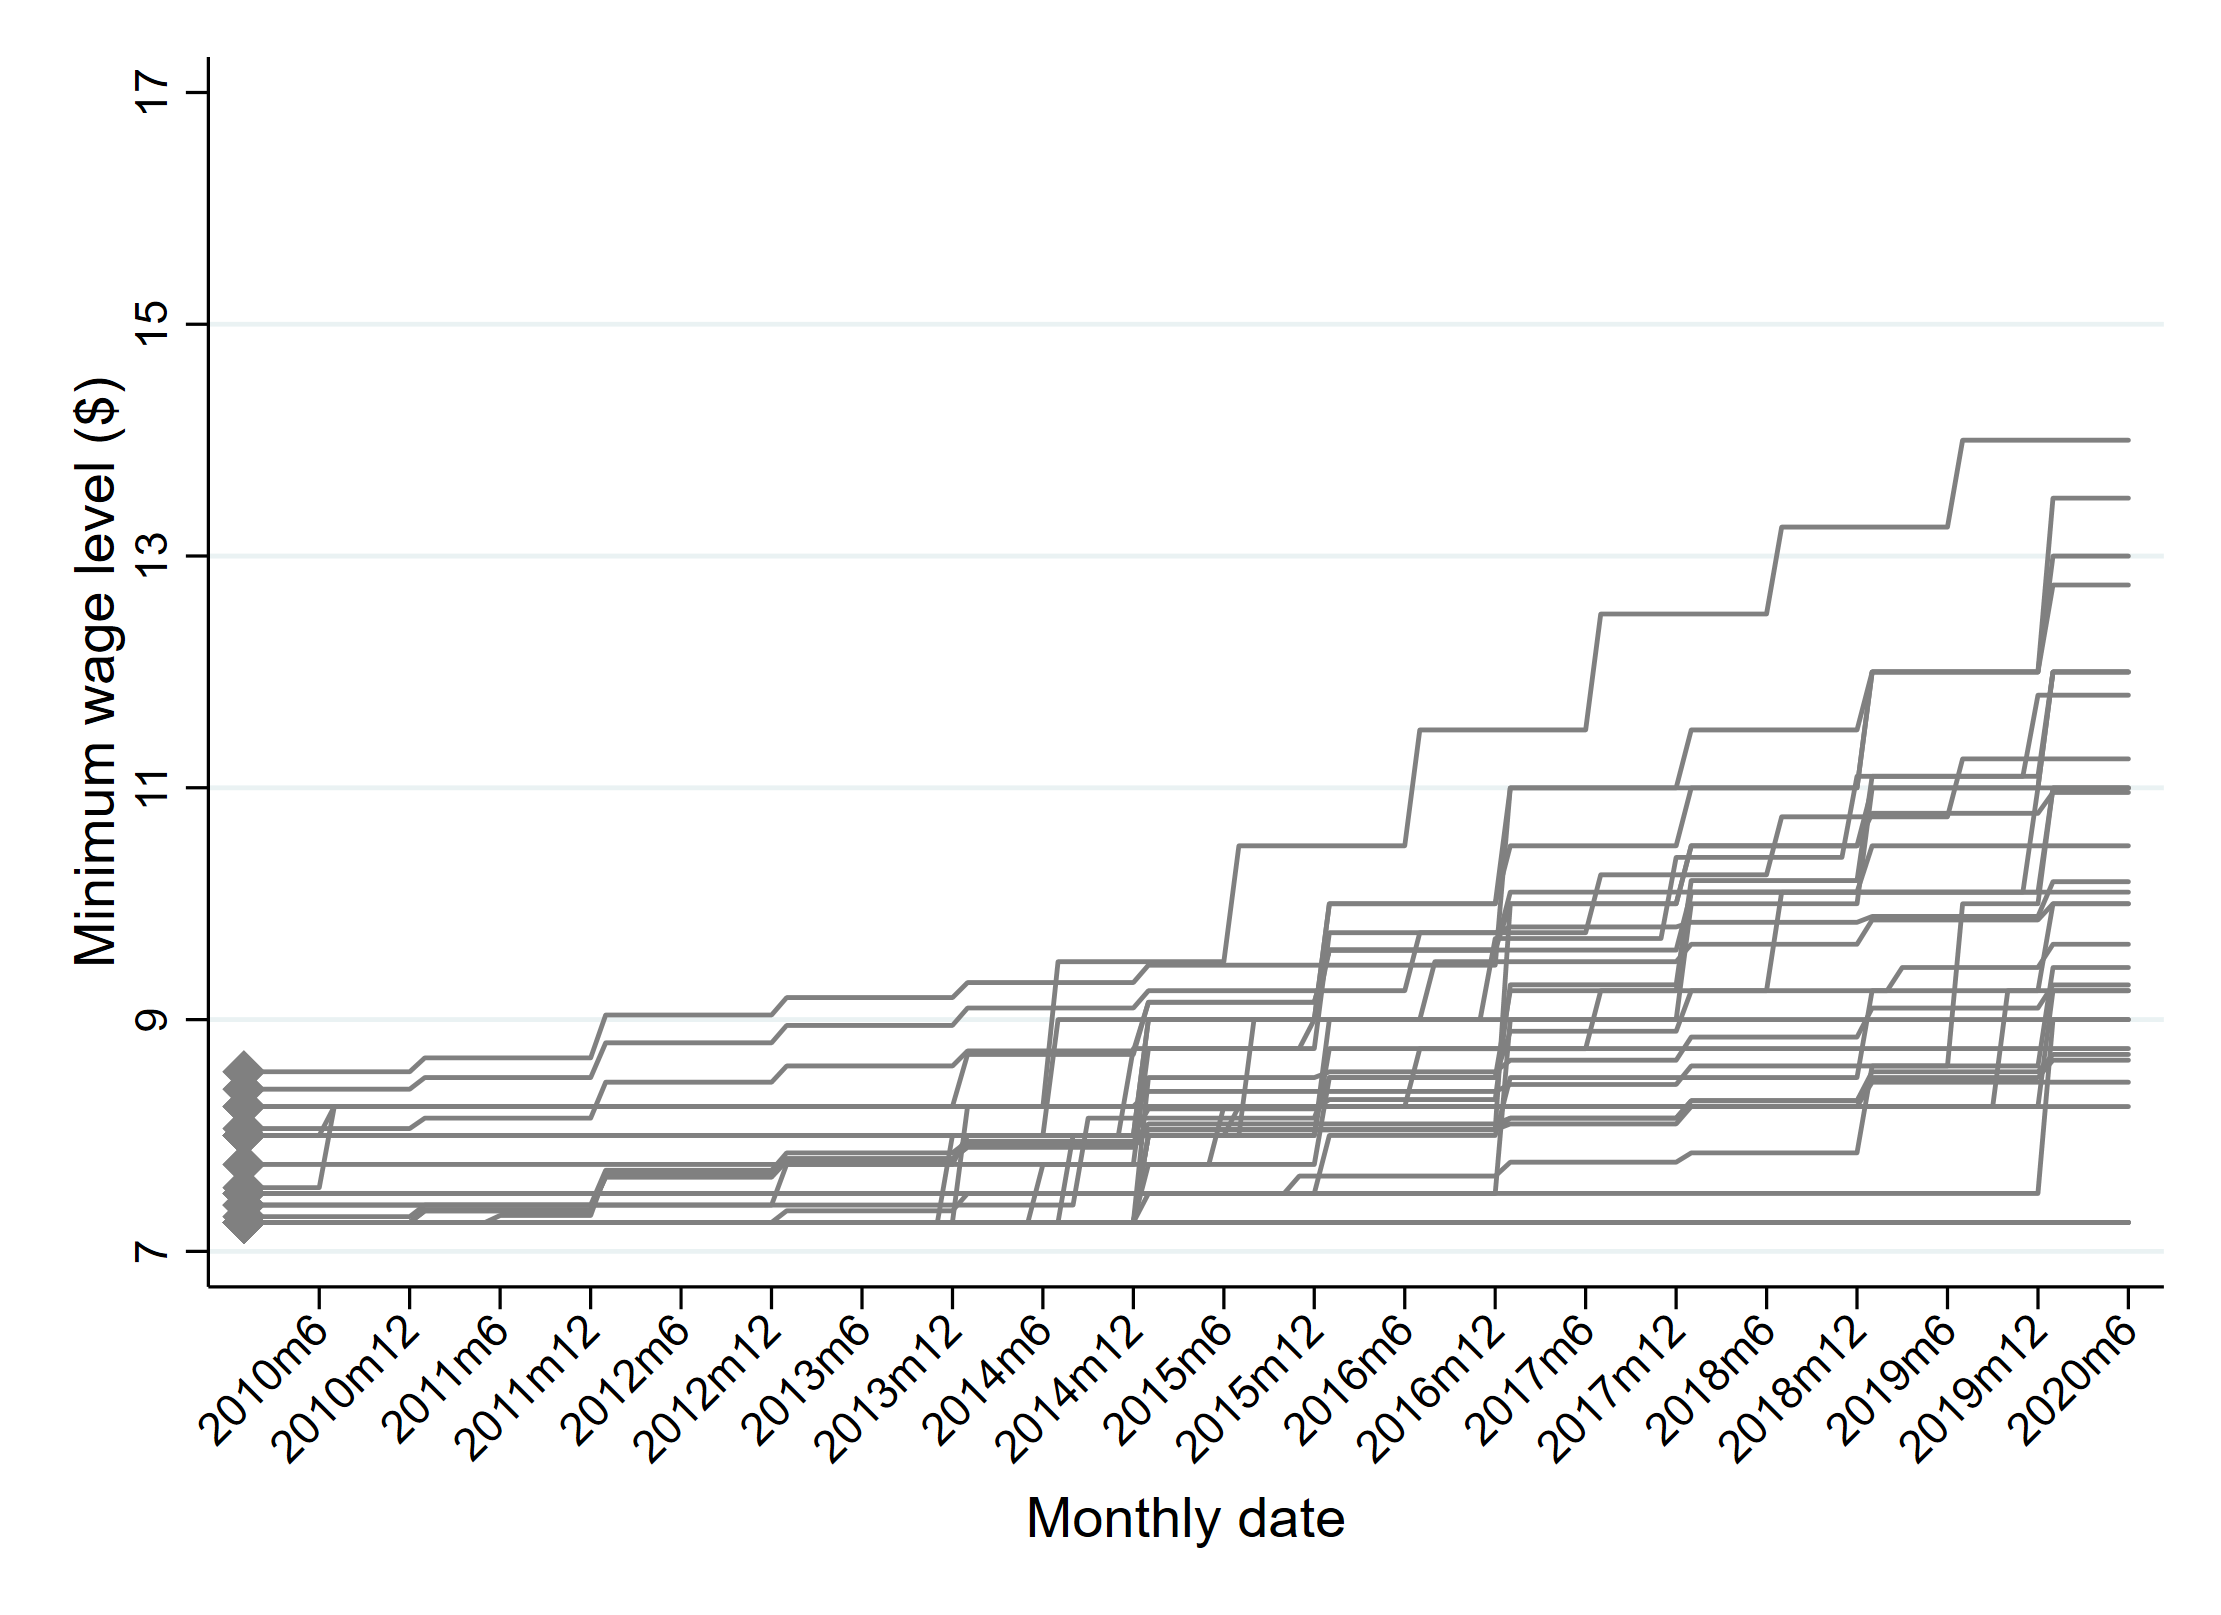
\includegraphics[width = \textwidth]
            {mw_US/output/state_mw_levels}
    \end{subfigure}\\
    \begin{subfigure}{.7\textwidth}
        \caption{Sub-state policies}
        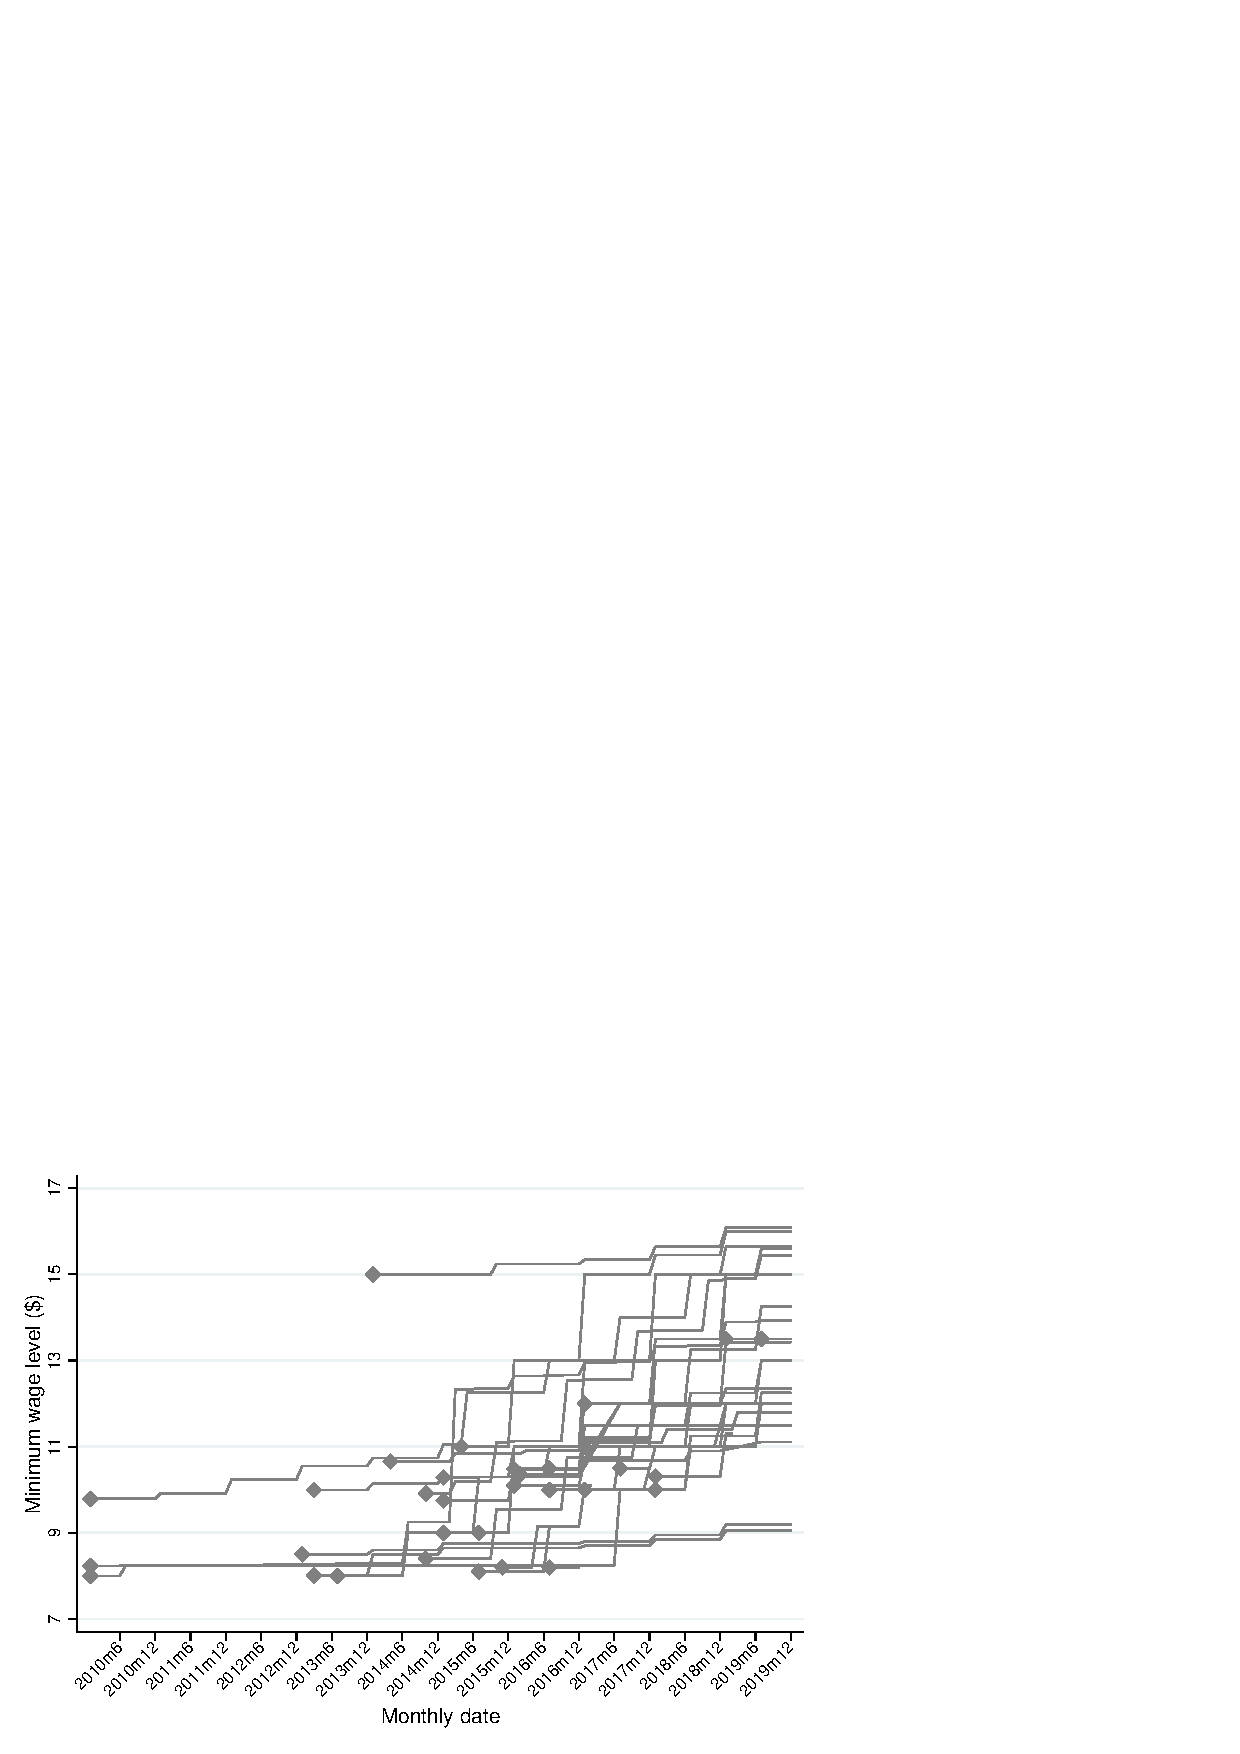
\includegraphics[width = \textwidth]
            {mw_US/output/local_mw_levels}
    \end{subfigure}

    \begin{minipage}{.95\textwidth} \footnotesize
        \vspace{3mm}
        Notes:
        Data are from the minimum wage panel described in Section 
        \ref{sec:data_mw_panel}.
        Lines show the levels of the minimum wage for jurisdictional policies 
        that were binding for at least one ZIP code inside them in some month 
        between January 2010 and December 2019.
        Diamonds indicate the first month the minimum wage policy became 
        operational within the same period.
        Panel (a) reports state level policies.
        Panel (b) reports sub-state level policies.
    \end{minipage}
\end{figure}
